\subsection{Background}
\subsubsection{K Nearest Neighbor graphs}
K nearest neighbor graph for a set of $n$ objects $P$ in a metric space (e.g., for a set of points in the plane with Euclidean distance) is a directed graph with $P$ being its vertex set and with directed edges from $p$ to all nodes $q \in P$ in a set of $k$ nearest neighbors set of $p$ (i.e., the distance from $p$ to $q$ is no larger than $k$th smallest distance from $q$ to any other object from $P$).

They can show a measure of the correlation between the degree of a node and that of its neighbors.
In many systems strong correlations are observed, and one distinguishes networks into assortative and disassortative.
A network is assortative if large (small) degree nodes tend to be linked with large (small) degree nodes.
Typical examples of assortative networks are social networks~\cite{information_or_social_network}.
A network is disassortative if large (small) degree nodes tend to be linked with small (large) degree nodes.
Biological and technological networks (like the Internet~\cite{lecture_sergei_maslov_internet}) are examples of disassortative networks.
On a directed graph one distinguishes between indegree (number of edges incoming to a node) and outdegree (number of edges outgoing from a node), so one can also test different types of correlations.

\subsubsection{Pearson Product-Moment correlation coefficient}

The Pearson product-moment correlation coefficient (or Pearson correlation coefficient, for short) is a measure of strength of linear association between two variables and is denoted by $r$ for samples and $\rho$ for populations.
Basically, it indicates how far away all the data points from the dataset are located to the line of best fit (how well the data points fit the new model/line of best fit).
Pearson correlation coefficient, $\rho$, represented with the following formula for populations:

$$ \rho_{X,Y} = \frac{cov(X,Y)}{\sigma_x \sigma_y}$$

Where $\sigma_X$ and $\sigma_Y$ are standard deviations of populations $X$ and $Y$ respectively and $cov(X,Y)$ is covariance between $X$ and $Y$.
It can be also represented as $r$, using the following formula for samples of size $n$:

$$r = \frac{\sum_{i=1}^{n} (X_i - \bar{X}) (Y_i - \bar{Y}) }
{ \sqrt{\sum_{i=1}^{n} (X_i - \bar{X})^2} \sqrt{\sum_{i=1}^{n} (X_i - \bar{X})^2} }$$

Where $\bar{X}$ and $\bar{Y}$ are mean values of samples from populations $X$ and $Y$.

Pearson correlation coefficient can take a range of values from +1 (inclusive) to -1 (inclusive).
A value of 0 indicates that there is no association between the two variables.
A value greater than 0 indicates a positive association; meaning, as the value of one variable increases, so does the value of the other variable.
A value less than 0 indicates a negative association; meaning, as the value of one variable increases, the value of the other variable decreases.

\clearpage
Exemplar Pearson correlation coefficients with graphical representation (and line of best fit) are shown in Figure~\ref{fig:pearson_graph}.

\begin{figure}[h!]
  \centering
  \captionsetup{justification=centering}
    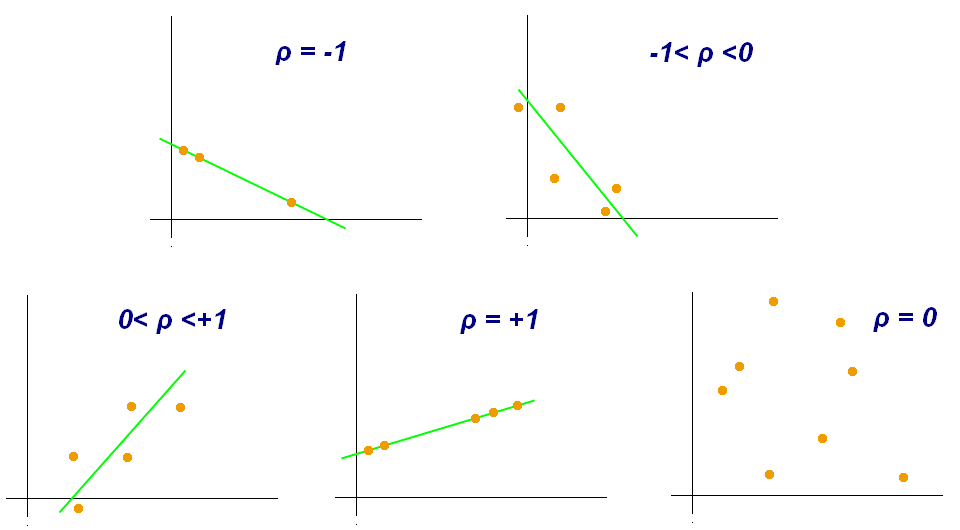
\includegraphics[width=0.8\textwidth]{images/pearson_graphs.png}
  \caption{Graphs showing dependence between graph points, assortativity coefficient and line of best fit.\cite{wiki_pearson}}
  \label{fig:pearson_graph}
\end{figure}

One more thing to note regarding Pearson correlation coefficient is that it does not represent the slope of the line of best fit.
Therefore, if you get a Pearson correlation coefficient of +1 this does not mean that for every unit increase in one variable there is a unit increase in another.
It simply means that there is no variation between the data points and the line of best fit what is illustrated in Figure~\ref{fig:pearson_graph_slope}:

\begin{figure}[h!]
  \centering
  \captionsetup{width=24pc, justification=centering}
    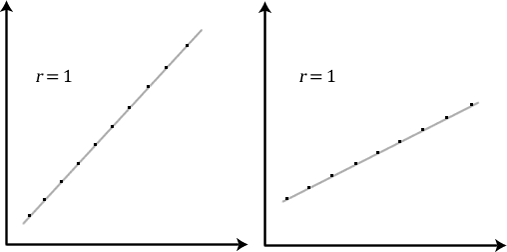
\includegraphics[width=0.55\textwidth]{images/pearson_graphs_slope.png}
  \caption{Graph showing independence of $r$ and slope of the line of best fit.}
  \label{fig:pearson_graph_slope}
\end{figure}

\subsubsection{Assortativity coefficient}
Assortativity coefficient is the Pearson correlation coefficient of degrees between connected nodes in k-NN graph.
With positive assortative coefficient $(0, 1>$, nodes tend to connect to other nodes that are similar.
With negative assortative coefficient $<-1, 0$, nodes tend to connect to nodes that are different (have different degrees).
Values close to $0$ indicate no tendency of nodes to connect to any other particular nodes (random connections).

\subsection{Problem definition}
The problem is to define whether there exists relation between parameter $k$ of kNN graph, that is its out-degree (number of outbound connections of each node in the graph) and assortativity coefficient in high dimensional datasets.
The conclusions from possible solutions to this problem may reveal whether nodes from real world datasets tend to connect to similar nodes or not.
Whether real world nodes tend to form groups of nodes with similar characteristic or rathere they tend to connect with different nodes.